\begin{figure}[!ht]
    \centering
    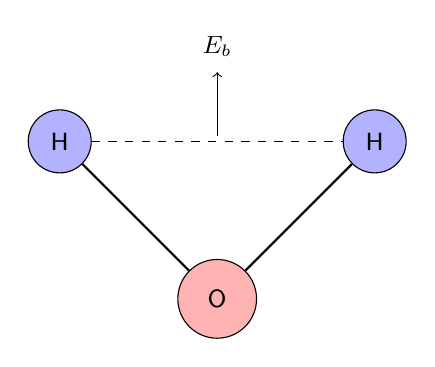
\begin{tikzpicture}[scale=2, font=\sansmath\sffamily, every node/.style={font=\sansmath\sffamily\small}]

% Nguyên tử Oxy
\node[circle, draw, fill=red!30, minimum size=1cm] (O) at (0,0) {O};

% Nguyên tử Hydro
\node[circle, draw, fill=blue!30, minimum size=0.8cm] (H1) at (-1,1) {H};
\node[circle, draw, fill=blue!30, minimum size=0.8cm] (H2) at (1,1) {H};

% Các liên kết
\draw[thick] (O) -- (H1);
\draw[thick] (O) -- (H2);

% Đường gạch giữa hai nguyên tử Hydro
\draw[dashed] (H1) -- (H2);

% Ghi chú E_b
\node (Eb) at (0,1.6) {$E_b$};

% Mũi tên nhỏ từ đường gạch lên E_b
\draw[->, shorten >=2pt, shorten <=2pt] (0,1) -- (Eb);

\end{tikzpicture}
    \caption{Lực liên kết}
\end{figure}
